\subsection{Linear Systems of Equations}

\begin{definition}[Linear Equation]
A \textbf{linear equation} with $n$ unknowns $x_1, x_2, \ldots, x_n$ is an equation of the form
\[
  a_1 x_1 + a_2 x_2 + \cdots + a_n x_n = b,
\]
where $a_1, a_2, \ldots, a_n, b \in \mathbb{R}$ are given constants.
\end{definition}

\begin{definition}[$m \times n$ Linear System]
An $m \times n$ \textbf{linear system} consists of $m$ linear equations in $n$ unknowns:
\[
  \begin{cases}
    a_{11}x_1 + a_{12}x_2 + \cdots + a_{1n}x_n = b_1 \\
    a_{21}x_1 + a_{22}x_2 + \cdots + a_{2n}x_n = b_2 \\
    \hspace{2em}\vdots \\
    a_{m1}x_1 + a_{m2}x_2 + \cdots + a_{mn}x_n = b_m
  \end{cases}
\]
\end{definition}

Any linear system has exactly one of three types of solution sets: no solution, exactly one solution, or infinitely many solutions. For a $2 \times 2$ system these correspond geometrically to two lines being parallel, intersecting, or identical.

\begin{center}
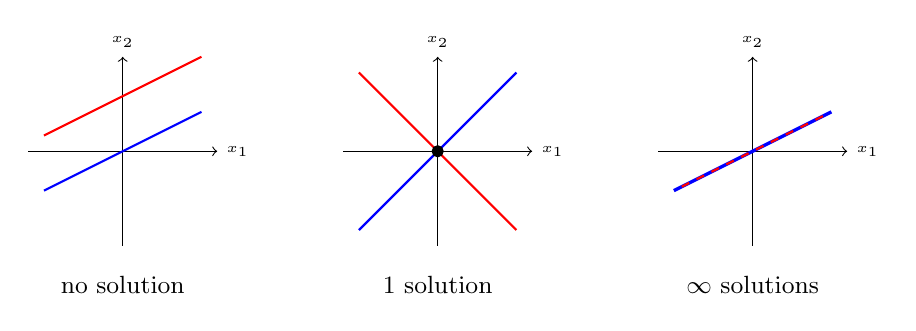
\begin{tikzpicture}
  % No solution: parallel lines
  \begin{scope}
    \draw[->] (-1.2,0)--(1.2,0) node[right,font=\tiny]{$x_1$};
    \draw[->] (0,-1.2)--(0,1.2) node[above,font=\tiny]{$x_2$};
    \draw[blue,thick] (-1,-0.5)--(1,0.5);
    \draw[red,thick]  (-1, 0.2)--(1,1.2);
    \node[font=\small] at (0,-1.7) {no solution};
  \end{scope}
  % 1 solution: intersecting lines
  \begin{scope}[xshift=4cm]
    \draw[->] (-1.2,0)--(1.2,0) node[right,font=\tiny]{$x_1$};
    \draw[->] (0,-1.2)--(0,1.2) node[above,font=\tiny]{$x_2$};
    \draw[blue,thick] (-1,-1)--(1,1);
    \draw[red,thick]  (-1,1)--(1,-1);
    \filldraw[black] (0,0) circle (2pt);
    \node[font=\small] at (0,-1.7) {$1$ solution};
  \end{scope}
  % Infinite solutions: same line
  \begin{scope}[xshift=8cm]
    \draw[->] (-1.2,0)--(1.2,0) node[right,font=\tiny]{$x_1$};
    \draw[->] (0,-1.2)--(0,1.2) node[above,font=\tiny]{$x_2$};
    \draw[blue,very thick] (-1,-0.5)--(1,0.5);
    \draw[red,dashed,thick] (-0.9,-0.45)--(0.9,0.45);
    \node[font=\small] at (0,-1.7) {$\infty$ solutions};
  \end{scope}
\end{tikzpicture}
\end{center}

\subsubsection*{Row Operations}

\begin{definition}[Elementary Row Operations]
The three \textbf{elementary row operations} on a linear system are:
\begin{enumerate}
  \item Multiply a row by a non-zero scalar.
  \item Interchange two rows.
  \item Replace a row with itself plus a scalar multiple of another row.
\end{enumerate}
Each operation produces an equivalent system (same solution set).
\end{definition}

\subsubsection*{Augmented Matrix and Row Reduction}

A system is conveniently represented by its \textbf{augmented matrix}
$\bigl[A \mid \mathbf{b}\bigr]$. Row operations are applied to this matrix to reach \textbf{triangular (row echelon) form}, after which the unknowns are solved by back-substitution.

\begin{example}
  Solve the $3 \times 3$ system
  \[
    \begin{cases}
      x_1 + 2x_2 - x_3 = 2 \\
      2x_1 + 3x_2 + x_3 = 9 \\
      3x_1 + 5x_2 + 2x_3 = 14
    \end{cases}
  \]

  Augmented matrix:
  \[
    \left[\begin{array}{ccc|c}
      1 & 2 & -1 & 2 \\
      2 & 3 &  1 & 9 \\
      3 & 5 &  2 & 14
    \end{array}\right]
    \begin{matrix} R_1 \\ R_2 \\ R_3 \end{matrix}
  \]

  Apply $R_2 \leftarrow R_2 - 2R_1$ and $R_3 \leftarrow R_3 - 3R_1$:
  \[
    \longrightarrow
    \left[\begin{array}{ccc|c}
      1 &  2 & -1 & 2 \\
      0 & -1 &  3 & 5 \\
      0 & -1 &  5 & 8
    \end{array}\right]
  \]

  Apply $R_3 \leftarrow R_3 - R_2$:
  \[
    \longrightarrow
    \left[\begin{array}{ccc|c}
      1 &  2 & -1 & 2 \\
      0 & -1 &  3 & 5 \\
      0 &  0 &  2 & 3
    \end{array}\right]
  \]

  The system is now in triangular form; solve $x_3$, then $x_2$, then $x_1$ by back-substitution.
\end{example}
